% Copyright 2004 by Till Tantau <tantau@users.sourceforge.net>.
%
% In principle, this file can be redistributed and/or modified under
% the terms of the GNU Public License, version 2.
%
% However, this file is supposed to be a template to be modified
% for your own needs. For this reason, if you use this file as a
% template and not specifically distribute it as part of a another
% package/program, I grant the extra permission to freely copy and
% modify this file as you see fit and even to delete this copyright
% notice. 

\documentclass[xcolor=table]{beamer}

\usepackage{ulem}
\usepackage{natbib}
\usepackage{multirow}
\usepackage[table,xcdraw]{xcolor}

% There are many different themes available for Beamer. A comprehensive
% list with examples is given here:
% http://deic.uab.es/~iblanes/beamer_gallery/index_by_theme.html
% You can uncomment the themes below if you would like to use a different
% one:
%\usetheme{AnnArbor}
%\usetheme{Antibes}
%\usetheme{Bergen}
%\usetheme{Berkeley}
%\usetheme{Berlin}
%\usetheme{Boadilla}
%\usetheme{boxes}
%\usetheme{CambridgeUS}
%\usetheme{Copenhagen}
%\usetheme{Darmstadt}
\usetheme{default}
%\usetheme{Frankfurt}
%\usetheme{Goettingen}
%\usetheme{Hannover}
%\usetheme{Ilmenau}
%\usetheme{JuanLesPins}
%\usetheme{Luebeck}
%\usetheme{Madrid}
%\usetheme{Malmoe}
%\usetheme{Marburg}
%\usetheme{Montpellier}
%\usetheme{PaloAlto}
%\usetheme{Pittsburgh}
%\usetheme{Rochester}
%\usetheme{Singapore}
%\usetheme{Szeged}
%\usetheme{Warsaw}

\addtobeamertemplate{navigation symbols}{}{%
    \usebeamerfont{footline}%
    \usebeamercolor[fg]{footline}%
    \hspace{1em}%
    \insertframenumber/\inserttotalframenumber
}

\title{Sentiment Analysis}

% A subtitle is optional and this may be deleted
\subtitle{Mining Opinions, Sentiments and Emotions}

\author{Van-Duyet LE (me@duyet.net)}
% - Give the names in the same order as the appear in the paper.
% - Use the \inst{?} command only if the authors have different
%   affiliation.

% \institute[Universities of Somewhere and Elsewhere] % (optional, but mostly needed)
% {
%   \inst{1}%
%   Department of Computer Science\\
%   University of Somewhere
%   \and
%   \inst{2}%
%   Department of Theoretical Philosophy\\
%   University of Elsewhere}
% - Use the \inst command only if there are several affiliations.
% - Keep it simple, no one is interested in your street address.

\date{06/2018}
% - Either use conference name or its abbreviation.
% - Not really informative to the audience, more for people (including
%   yourself) who are reading the slides online

\subject{NLP}
% This is only inserted into the PDF information catalog. Can be left
% out. 

% If you have a file called "university-logo-filename.xxx", where xxx
% is a graphic format that can be processed by latex or pdflatex,
% resp., then you can add a logo as follows:

% \pgfdeclareimage[height=0.5cm]{university-logo}{university-logo-filename}
% \logo{\pgfuseimage{university-logo}}

% Delete this, if you do not want the table of contents to pop up at
% the beginning of each subsection:
\AtBeginSubsection[]
{
  \begin{frame}<beamer>{Outline}
    \tableofcontents[currentsection,currentsubsection]
  \end{frame}
}

% Let's get started
\begin{document}

\begin{frame}
  \titlepage
\end{frame}

\begin{frame}{Outline}
  \tableofcontents
  % You might wish to add the option [pausesections]
\end{frame}

% Section and subsections will appear in the presentation overview
% and table of contents.
\section{Introduction}

\begin{frame}{Introduction}
    \begin{block}{Sentiment}
        \begin{itemize}
            \item Sentiment = feelings
            \begin{itemize}
                \item Attitudes
                \item Emotions
                \item Opinions
            \end{itemize}
            \item Subjective impressions, not facts.
            \item For/against, like/dislike, good/bad, etc.
        \end{itemize}
    \end{block}

    \pause
    \begin{block}{Sentiment analysis}
    is contextual mining of text which identifies and extracts subjective information in source material. \\
    Using NLP, statistics, or machine learning methods to extract, identify, or otherwise characterize the sentiment content of a text unit.
    \end{block}
\end{frame}

\subsection{Sentiment Analysis Application}

\begin{frame}{Sentiment Analysis Application}
    \begin{itemize}
        \item In the past, an organization or a business \sout{conducted surveys}, \sout{opition polls} and \sout{focus groups}.
        \begin{itemize}
            \item Helping a \textbf{business} to understand the social sentiment of their brand, product or service while monitoring online conversations.
        \end{itemize}
        
        \pause
        \item Governments can easily obtain public opitions about their policies and measure the pulses of other nations.
        
        \pause
        \item Opinionated documents of internal data: customer feedback, email, call centers, results of surveys, etc.
        
        \pause
        \item Consumer products \cite{sadikov2009blogs}, healthcare \cite{khanhealthcare}, tourism, and financial services\cite{devitt2007sentiment} to social events and political elections\cite{o2010tweets}\cite{tumasjan2010predicting}.
        
    \end{itemize}
\end{frame}


\begin{frame}{Sentiment Analysis Application}

    \begin{figure}[ht]
        \begin{minipage}[b]{0.45\linewidth}
            \centering
            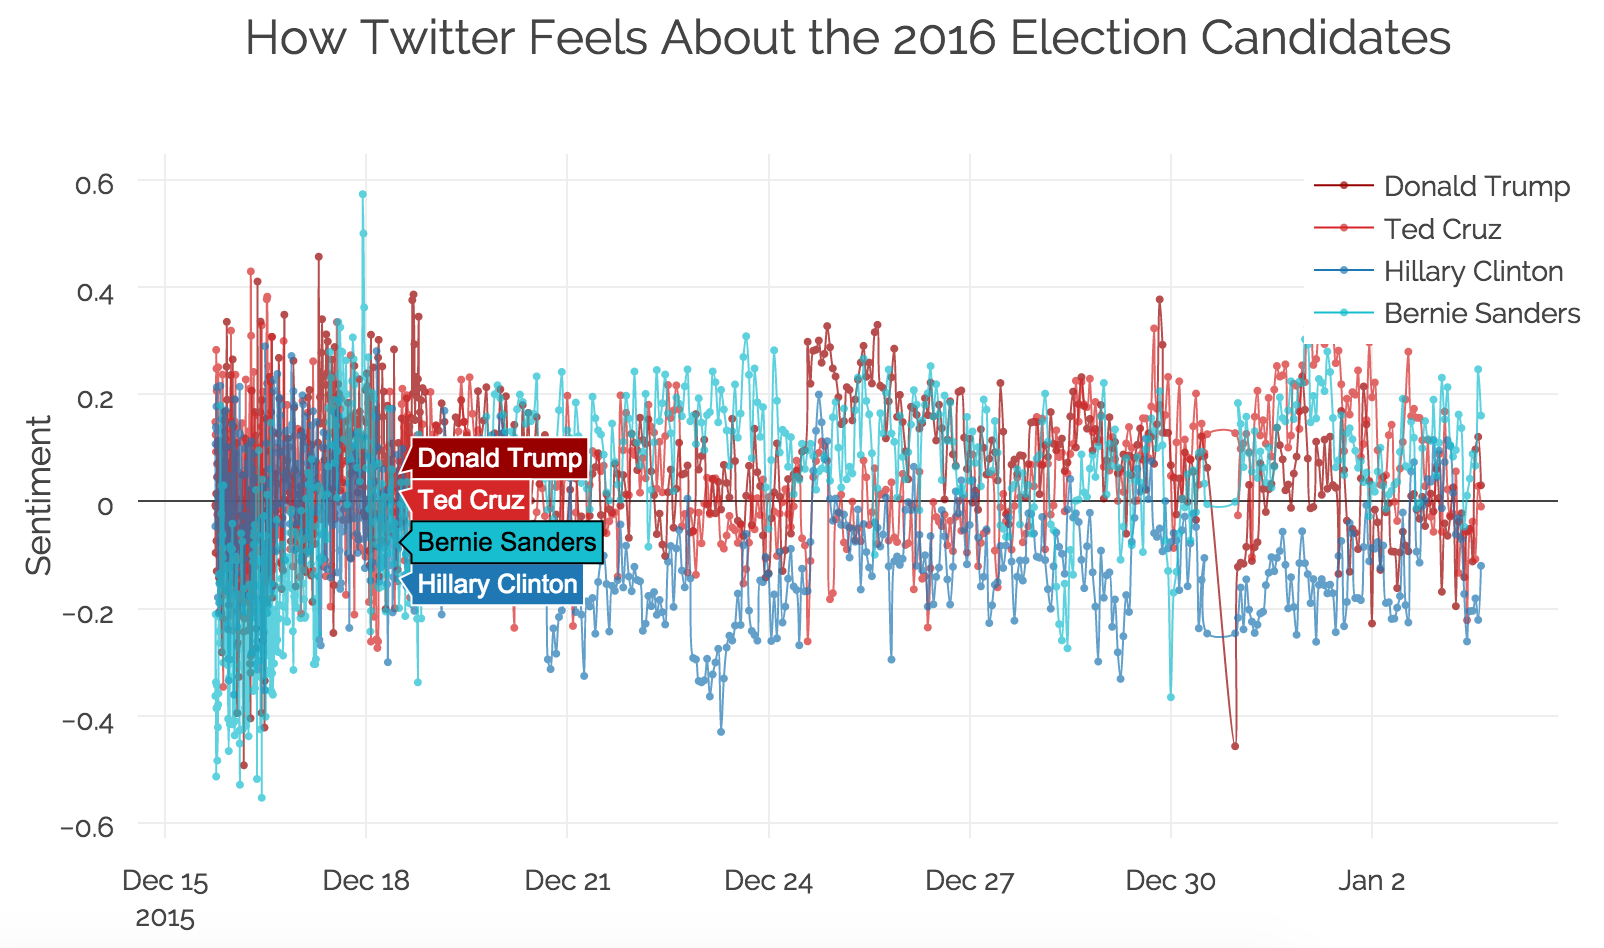
\includegraphics[width=\textwidth]{img/SA-election.png}
            \caption{US Election 2016}
            \label{fig:a}
        \end{minipage}
        \hspace{0.5cm}
        \begin{minipage}[b]{0.45\linewidth}
            \centering
            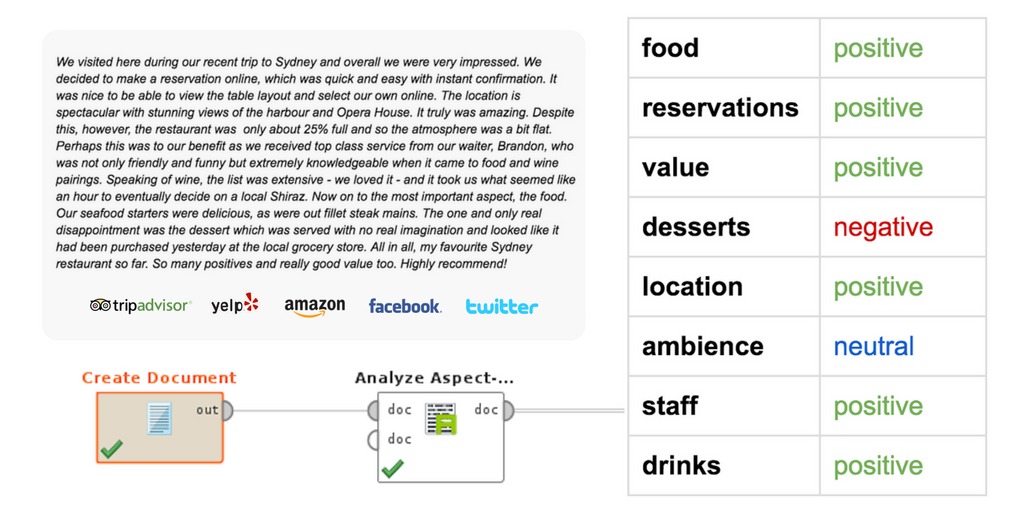
\includegraphics[width=\textwidth]{img/SA-aspect.png}
            \caption{SA for customer reviews}
            \label{fig:b}
        \end{minipage}
    \end{figure}

\end{frame}




\subsection{Sentiment Analysis Research}

\begin{frame}{Different Levels of Analysis}
    Sentiment Analysis research has been mainly carried out at three levels of granularity:
    \begin{itemize}
        \item \textbf{Document level}
            \begin{itemize}
                \item e.g. given a product review, overall positive or negative.
                \item Assuming that each document expresses opinions on a single entity.
            \end{itemize}
        
        \item \textbf{Sentence level}
        \item \textbf{Aspect level}
            \begin{itemize}
                \item discover sentiment on entities and/or their aspects.
                \item e.g. \textit{"I like the iPhone X", "Although the service is not great, I still love this hotel."}
            \end{itemize}
    \end{itemize}
\end{frame}

% \section{The Problem of Sentiment Analysis}
% \subsection{Definition of Opinion}
% \subsection{Definition of Opinion Summary}
% \subsection{Affect, Emotion and Mood}

\section{Document Sentiment Classification}

\begin{frame}{Document Sentiment Classification}
    \begin{itemize}
    \item \textit{Document sentiment classification} detects the \textbf{overall opinion or sentiment} expressed in a document.
    \item It is perhaps the most extensively studied topic in the field of SA especially in its early days (see surveys by Pang and Lee, 2008 \cite{pang2008opinion}; Liu, 2012 \cite{liu2012sentiment})
    \item It treat sentiment classification as \textbf{a traditinal text classification problem}.
    \item It \textbf{not} concerned the \textbf{targets} of sentiment or opinion.
    \end{itemize}
    
    \begin{exampleblock}{Assumption}
    The opinion document \texttt{d} expresses opinions on a single entity \texttt{e} and contains opinions from a single opinion holder \texttt{
    h}
    \end{exampleblock}
    
\end{frame}

\begin{frame}{Document Sentiment Classification}
    \begin{itemize}
    \item \textbf{Holds well for} online reviews of products or services \\ (usually focus on single product or serice).
    \item \textbf{No meaningful for} blog posts, forum discussion \\ (multiple opinions, multiple entities or compares).
    \end{itemize}
    
\end{frame}



\begin{frame}{Document Sentiment Classification}
    \begin{enumerate}
        \item Supervised Sentiment Classification
            \begin{enumerate}
                \item Using Machine Learning Algorithms
                \item Using a Custom Score Function
            \end{enumerate}
        \item Unsupervised Sentiment Classification
            \begin{enumerate}
                \item Using Syntactic Patterns and Web Search
                \item Using Sentiment Lexicons
            \end{enumerate}
        \item Sentiment Rating Prediction
        \item Cross-Domain Sentiment Classification
        \item Cross-Language Sentiment Classification
        \item Emotion Classification of Documents
        
    \end{enumerate}
    
\end{frame}

\begin{frame}{1.1 Classification Using Machine Learning Algorithms}
    Any existing supervised learning method can be directly applied, such as Naive Bayes or SVM \cite{joachims1999transductive} \cite{cristianini2000introduction} \cite{pang2002thumbs}.
    
    \pause
    \textbf{Features engineering:}
    \begin{itemize}
        \item \textit{Terms and their frequency} highly effective, TFIDF weighting can be applied too.
        \item \textit{Part of speech (POS)}
        \item \textit{Sentiment words annd phrases} e.g. \textit{good, wonderful, ...} are positive sentiment words.
        \item \textit{Rules of opinion} using other constructs or language compositions.
        \item \textit{Sentiment shiters} expressions that are used to change sentiment orientations (e.g. \textit{"I don't like you"} is neg, although the word \textit{like} is pos.
        \item \textit{Syntactic dependency}
    \end{itemize}
\end{frame}


\begin{frame}{1.2 Classification Using a Custom Score Function}
    \begin{itemize}
        \item Customized techniques specifically for sentiment classification or reviews.
    
        \item Example is the score function of Dave et al \cite{dave2003mining}. \\
        
        \begin{figure}
            \centering
            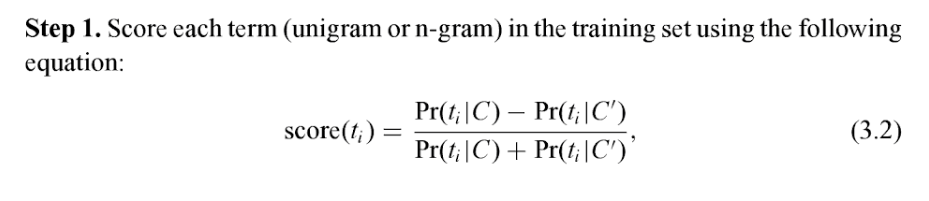
\includegraphics[width=0.7\textwidth]{img/funcs-1.PNG} \hfill
            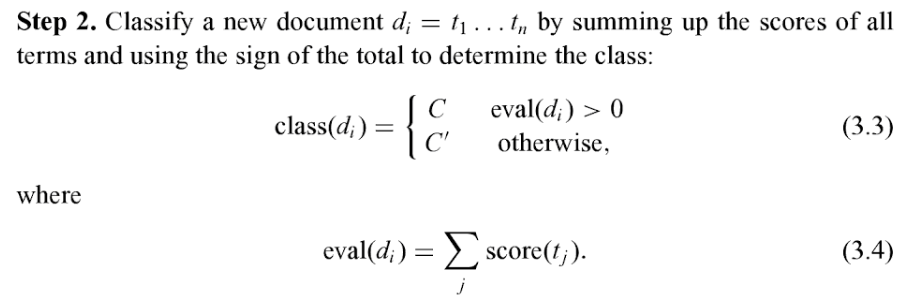
\includegraphics[width=0.7\textwidth]{img/funcs-2.PNG}
        \end{figure}
        
        
    \end{itemize}
\end{frame}


\begin{frame}{2. Unsupervised Sentiment Classification}
    \begin{figure}
        \centering
        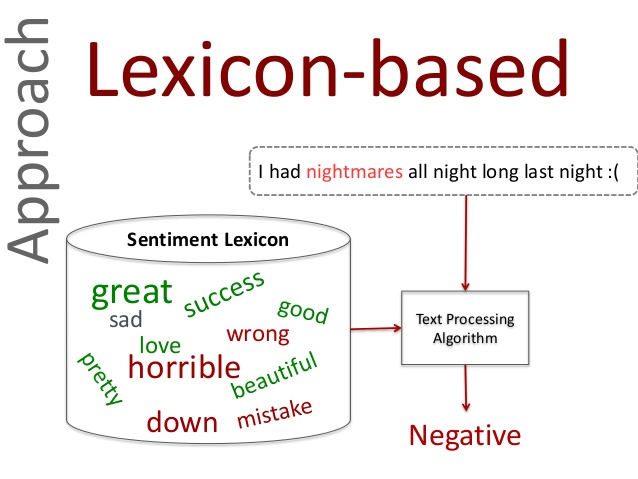
\includegraphics[width=0.6\textwidth]{img/lexi1.jpg}
        \caption{ Staano\footnote{\url{https://www.slideshare.net/Staano/senticircles-for-contextual-and-conceptual-semantic-sentiment-analysis-of-twitter}}}
    \end{figure}
\end{frame}


\begin{frame}{2. Unsupervised Sentiment Classification (continue)}
    \begin{figure}
        \centering
        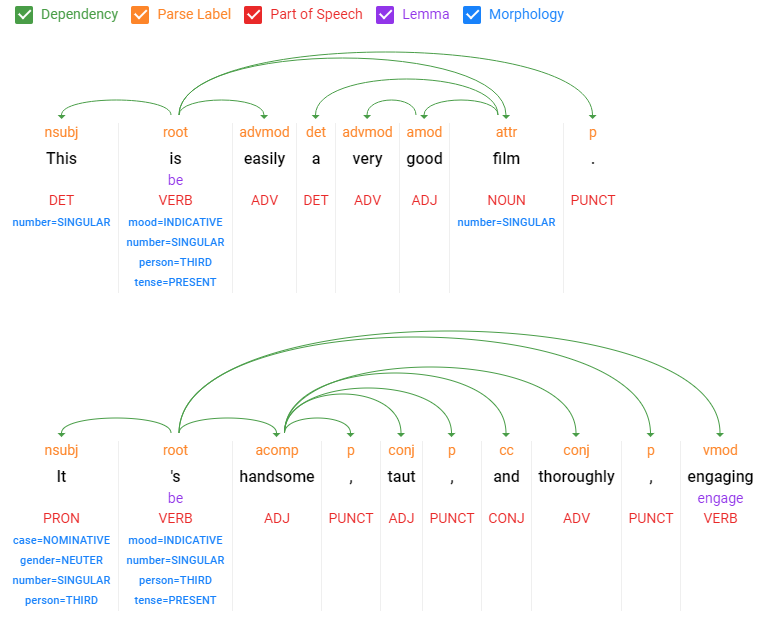
\includegraphics[width=0.9\textwidth]{img/lexi-parse.PNG}
    \end{figure}
\end{frame}


\begin{frame}{2. Unsupervised Sentiment Classification (continue)}
    \begin{figure}
        \centering
        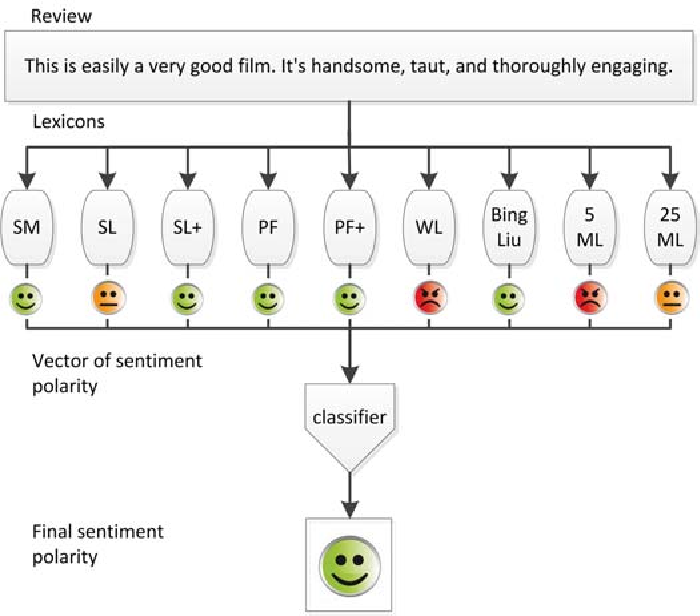
\includegraphics[width=0.5\textwidth]{img/lexi.png}
        \caption{Augustyniak, Lukasz et al \cite{Augustyniak2014SimplerIB}. “Simpler is better? Lexicon-based ensemble sentiment classification beats supervised methods.” 2014 IEEE/ACM International Conference on Advances in Social Networks Analysis and Mining (ASONAM 2014) (2014): 924-929.}
    \end{figure}
\end{frame}


\begin{frame}{3. Classification Using Rating Prediction}
    \begin{itemize}
        \item Using rating score (e.g., 1-5 stars) of reviews
        \begin{itemize}
            \item Pang and Lee, 2005 \cite{pang2005seeing} using SVM regression and SVM multiclass OVA.
            \item Long et al. 2010 \cite{long2010review}: Bayesian network classifier
        \end{itemize}
    \end{itemize}
\end{frame}

\begin{frame}{4. Cross-Domain Sentiment Classification}
    \begin{itemize}
        \item Words and even langage constructs used to expressing opinions in different domains can be quite different.
        \item Existing research is mainly based on two settings:
        \begin{itemize}
            \item a small amount of labeled training data for the new domain (Aue and Gamon, 2005 \cite{aue2005customizing}).
            \item No labeled data for the new domain (Blitzer et al., 2007\cite{blitzer2007biographies}; Tan et al., 2007\cite{tan2007novel})
        \end{itemize}
    \end{itemize}
\end{frame}

\begin{frame}{5. Cross-Language Sentiment Classification}
    Motivations:
    \begin{itemize}
        \item Apply existing SA (done and good) to another languages.
        \item Many apps, companies want to know and compare consumer opinions in different countries.
    \end{itemize}
    \pause
    
    
    Some approachs:
    \begin{itemize}
        \item Wan (2008)\cite{wan2008using} translate each Chinese review into English using multiple translators, classify and sums up sentiment score.
        
        \item Wan (2009)\cite{wan2009co} using co-training method (SVM) and Wan (2013)\cite{wan2013co} based on co-training idea, using co-regresion method.
        
        \item Boyd-Graber and Resnik (2010)\cite{boyd2010holistic} extended SLDA to MLSLDA.
    \end{itemize}
    
\end{frame}

\begin{frame}{6. Emotion Classification of Documents}
    Emotion Classification of Documents
\end{frame}



\section{Sentence Sentiment Classification}
\subsection{Overview}

\begin{frame}{Sentence Sentiment Classification - Overview}
    \begin{itemize}
        \item Same with document level.
        \item The goal is to classify positive, negative or neutral\text{*}. \\
        \begin{figure}
            \centering
            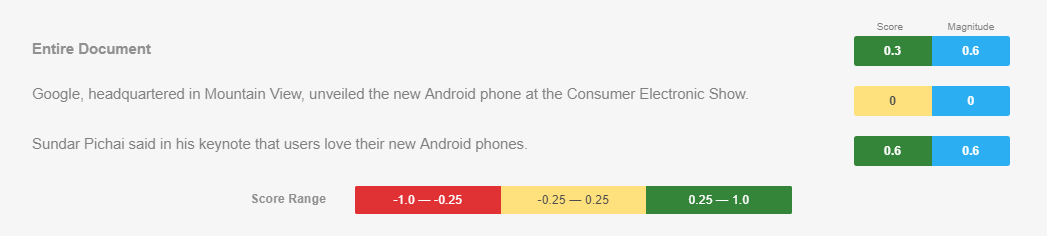
\includegraphics[width=0.8\textwidth]{img/sentence-level.png}
        \end{figure}
        \pause
        \item Can be solved either as \textbf{(1) a three-class} classification or as \textbf{(2) two separate two-class} classification.
    \end{itemize}
    
\end{frame}

\subsection{Subjectivity classification}
\begin{frame}{Subjectivity classification}

    \textbf{(2) two separate two-class} classification:
    \begin{enumerate}
        \item First step: classify whether a sentence expresses an opinion (\textit{subjectivity classification}).
        \item Second step: classifies those opinion sentences into positive and negative classes.
    \end{enumerate}
    
\begin{table}[]
\centering
\begin{tabular}{|c|c|}
\hline
\textbf{Subjectivity Analysis} & \textbf{Sentiment Analysis}                             \\ \hline
                               & \cellcolor[HTML]{009901}Positive                        \\ \cline{2-2} 
\multirow{-2}{*}{Subjective}   & \cellcolor[HTML]{F56B00}{\color[HTML]{333333} Negative} \\ \hline
Objective                      & \cellcolor[HTML]{ECF4FF}Neutral                         \\ \hline
\end{tabular}
\end{table}

\end{frame}


\begin{frame}{Subjectivity classification}
    \textbf{Subjectivity classification} classifies sentences into two classes, subjective and objective (Wiebe et al., 1999 \cite{wiebe1999development}).\\
    
    Most approaches are based on supervised or unsupervised learning:
    \begin{itemize}
        \item Weibe et al. (1999) \cite{wiebe1999development} Naive Bayes
        \item Yu and Hatzivassiloglou (2003) \cite{yu2003towards} sentence similarity and Naive Bayes
        \item Pang and Lee (2004) \cite{pang2004sentimental} mincut-based
    \end{itemize}
\end{frame}

\subsection{Sentence Sentiment Classification}
\begin{frame}{Sentence Sentiment Classification}
    Supervised learning again can be applied to solve the problem, and so can lexicon-based methods.
    
    \begin{itemize}
        \item Dealing with Conditional Sentences
        \item Dealing with Sarcastic Sentences
        \item Using Discourse Information for Sentiment Classification
        \item Emotion Classification of Sentences
    \end{itemize}
\end{frame}

\begin{frame}{Dealing with Conditional Sentences}
    Conditional sentences are sentences that describe implications or hypothetical situations and their consequences.
    
    \begin{example}
    \textit{"If your phone is not good, buy this iPhone"} \\
    \end{example}
    
    Narayanan et al. (2009) \cite{narayanan2009sentiment} using a set of linguistic features.
    
    \begin{figure}
        \centering
        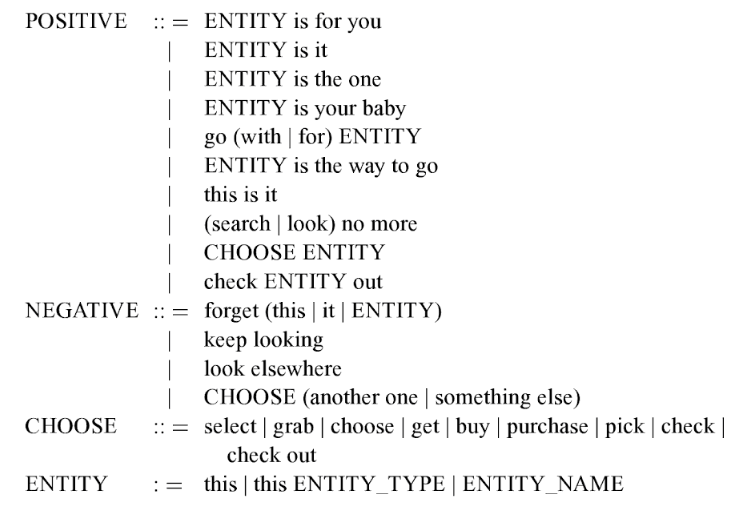
\includegraphics[width=0.7\textwidth]{img/SA-cond.PNG}
    \end{figure}
\end{frame}

\begin{frame}{Dealing with Sarcastic Sentences}
    Sarcasm is a sophisticated form of speech act in which the speakers or the writers say or write the opposite of what they mean.
    
    \begin{example}
        \textit{"The Earth is full. Go home."} \\
        \textit{"Don't bother me. I'm living happily ever after."}
    \end{example}
    
    \begin{itemize}
        \item Tsur et al. (2010) \cite{davidov2010semi} uses a small set of labeled sentences (seeds) and expands through web search.
        \item González-Ibánez (2011) studied in Twitter data to distinguish sarcastic and nonsarcastic tweets (SVM, LR), they used unigrams and some dict-based information.
    \end{itemize}
    
\end{frame}

\begin{frame}{Discussion}
    \begin{itemize}
        \item Sentence-level classifcation only suiable for simple sentences with a single opinion.
        \item Cannot deal with opinions in comparative sentences.
        \begin{itemize}
            \item E.g. \textit{"X is better than Y"}
        \end{itemize}
    \end{itemize}
\end{frame}

\section{Aspect Sentiment Classification}

\subsection{Overview}
\begin{frame}{Aspect Sentiment Classification}
    Aspect Sentiment (or entity-based sentiment analysis).
    
    \begin{example}
    \begin{itemize}
        \item \textit{"iPhone is great"}
        \begin{itemize}
            \item \textit{iPhone} is entity, aspect is \textit{GENERAL}
        \end{itemize}
        
        \item \textit{"iPhone's voice is great"}
        \begin{itemize}
            \item \textit{iPhone} is entity, aspect is \textit{voice quality}
        \end{itemize}
    \end{itemize}
    \end{example}
\end{frame}

\begin{frame}{Aspect Sentiment Classification}
    Two tasks:
    \begin{enumerate}
        \item Aspect extraction
        \item Aspect sentiment classification
    \end{enumerate}
\end{frame}

\subsection{Aspect Extraction}
\begin{frame}{Aspect Extraction}
    \begin{example}
        \textit{The sound from this iPhone X phone is great} \\
        \textit{Girls from A is so beautiful}
    \end{example}
    
    The entities are \textit{iPhone X} and \textit{A}, the aspects are \textit{sound} and \textit{girls}.
    \pause
    
    \begin{block}{Approaches }
        There are four main approaches to extracting explicit aspects:
        \begin{enumerate}
            \item Extraction by finding frequent nouns and noun phrases.
            \item Extraction by exploiting syntactic relations:
            \begin{enumerate}
                \item Syntactic dependencies depicting opinion and target relations.
                \item Lexico-syntactic patterns recoding entity and part/attribute relations.
            \end{enumerate}
            \item Extracting using supervised learning.
            \item Extracting using topic models.
        \end{enumerate}
    \end{block}
\end{frame}

\subsection{Aspect Sentiment Classification}
\begin{frame}{Aspect Sentiment Classification (ASC)}
    ASC has two main approaches:
    \begin{enumerate}
        \item The supervised learning approach
        \item The unsupervised lexicon-based approach
    \end{enumerate}
\end{frame}

\begin{frame}{1. The supervised learning approach}
    \begin{itemize}
        \item Jiang et al. (2011) \cite{jiang2011target} uses syntactic parse tree to generate a set of target-dependent features.
        \item Boiy and Moens (2009) \cite{boiy2009machine} computed the feature weight for each word feature based on \texttt{distance(word,\ target\_aspect)}
    \end{itemize}
\end{frame}

\begin{frame}{2. The unsupervised lexicon-based approach}
    TBD
\end{frame}

% All of the following is optional and typically not needed. 
\appendix
\section<presentation>*{\appendixname}
\subsection<presentation>*{Ref}

\begin{frame}[allowframebreaks]
  \frametitle<presentation>{Ref}
    
\bibliographystyle{unsrt}
\bibliography{ref}
 
 
\end{frame}

\end{document}


